% ARPEGOS:  Automatized Roleplaying-game Profile Extensible Generator Ontology based System %
% Author : Alejandro Muñoz Del Álamo %
% Copyright 2019 %

% Section 2.3: Propuesta %

\section{Propuesta} \label{Propuesta}
Tras analizar el estado del arte, y destacar algunos de los aspectos negativos de éste, lo que prosigue es diseñar una 
propuesta que permita recoger las mejores ideas de las herramientas actuales, y que además pueda dar solución a los 
problemas comentados en el apartado \ref{Critica_Estado_Arte} (\textit{Crítica al estado del arte}). \medskip

\subsection{Plataforma} \label{Plataforma}
En primer lugar, se debe considerar cuál será la plataforma en la que se implementará la aplicación, puesto que es la base 
sobre la que se realiza el desarrollo, y que condiciona las herramientas que se pueden utilizar para la elaboración del proyecto. 
\medskip

Como se puede apreciar en la sección \ref{Estado_Arte} (\textit{Estado del arte}), muchas de las aplicaciones existentes 
se desarrollan en entornos móviles, lo que supone que la aplicación pueda ser accesible desde cualquier sitio. Por otro lado, 
se considera una opción plausible el poder extender la aplicación a otros entornos, tales como sistemas de sobremesa, o el entorno 
web. Teniendo todo esto en consideración, se ha tomado la decisión de realizar una \textbf{aplicación móvil}, haciendo uso de 
\textbf{herramientas de desarrollo multiplataforma}, de manera que en un futuro sea posible extender el proyecto a otras plataformas.

\subsection{Arquitectura} \label{Arquitectura}
Después de seleccionar la plataforma principal de desarrollo, el siguiente paso es definir la arquitectura de la aplicación, 
que hace referencia a \textit{“la estructura general de este y a las formas en las que ésta da integridad conceptual a un 
sistema.”} \autocite*{Shaw1995}. Como explica Cardacci \autocite*{Addati2013}, con el tiempo se han ideado una amplia 
variedad de formas arquitectónicas, con el objetivo de separar los diferentes desafíos que plantea el desarrollo de software 
conceptualmente, y lograr cierto grado de independencia entre los elementos que componen el software, de manera que los cambios 
realizados en uno no tenga efecto en el resto. \medskip

De entre todas las posibilidades existentes, hemos optado por utilizar el patrón \textit{Modelo-Vista-Modelo de Vista} (\textbf{MVVM})
\autocite*{MicrosoftMVVM}, que separa el software en tres componentes: \textit{modelo}, \textit{modelo de vista} y \textit{vista}, cuyo 
esquema queda representado en la figura \ref*{mvvm}.\medskip

\begin{figure}[H]
    \centering
    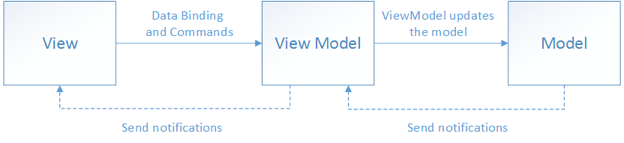
\includegraphics[width=10cm]{Images/mvvm.png}
    \caption{Patrón MVVM: \textit{Modelo-Vista-Modelo de Vista}. 
    Extraído de \textit{Microsoft Docs} \autocite*{MicrosoftMVVM}}
    \label{mvvm}
\end{figure}
\newpage
\subsection{Modelo de datos} \label{Modelo_Datos}
Como definen Pérez y Gardey \autocite*{Perez2017}, un modelo de datos es un esqueleto estructural que permite organizar 
y documentar la información. Esta estructura, presente en la figura \ref*{dataModel}, busca definir el acceso y el almacenamiento de los datos de forma 
unívoca, de manera que permitan la comunicación entre las aplicaciones que hagan uso de los datos del modelo. \medskip

\begin{figure}[H]
    \centering
    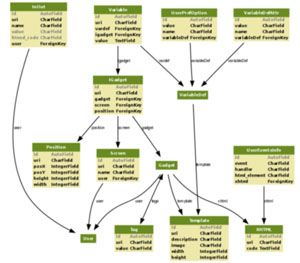
\includegraphics[width=5cm]{Figures/modelo_datos.jpg}
    \caption{Esquema de un modelo de datos. Extraído de \textit{definición.de} \autocite*{Perez2017}}
    \label{dataModel}
\end{figure}

Para este proyecto hace falta un modelo de datos que permita representar diversos mundos, y establecer relación entre sus elementos.
Por ello, se ha tomado la decisión de plantear un modelo \textbf{ontológico}. Citando a Muñoz y Aguilar \autocite*{Munoz2009}, 
\textit{“una ontología es una base de datos que describe los conceptos del mundo en un dominio específico, algunas de sus 
propiedades y cómo estos conceptos se relacionan entre sí”}. \autocite*{Munoz2009}
 
